%!TEX program = xelatex
%!TEX TS-program = xelatex
%!TEX encoding = UTF-8 Unicode

\documentclass[a4paper]{article}
\usepackage[UTF8, heading = false, scheme = plain]{ctex}
\usepackage{graphicx}
\usepackage{cite}
\usepackage{geometry}
\geometry{left=2.0cm, right=2.0cm, top=2.5cm, bottom=2.5cm}
\usepackage[colorlinks,linkcolor=red,anchorcolor=blue,citecolor=green]{hyperref}
\usepackage{subfig}
\usepackage{caption}
\captionsetup{font={scriptsize}}

\renewcommand\figurename{图}

\makeatletter
\let\@afterindentfalse\@afterindenttrue
\@afterindenttrue
\makeatother
\setlength{\parindent}{2em}  

\linespread{1.4}
\setlength{\parskip}{0.5\baselineskip}

\title{学习汇报\\第十一周}
\author{熊凯亚}
\date{\today}

\begin{document}
\maketitle
\section{回顾}
PATE中教师模型在互不相交的训练数据集上分别训练自己独立的模型,这些训练数据有可能是敏感数据。PATE使用教师模型聚集的共识答案以黑盒的方式来监督训练学生模型。然而原始的PATE\cite{Papernot2016SemisupervisedKT}只在MNIST上做了实验,并没有在大量实验数据的情况下做实验验证其可行性。
本文主要讲了
\begin{itemize}
\item 在原有PATE方案基础上对大量数据集进行验证。
\item 改善了原有PATE方案中教师模型的聚集机制。
\item 本方案只需添加更少的噪声即可保护隐私。
\end{itemize}

\subsection{聚集机制}

在PATE中,聚集机制主要是将拉普拉斯噪声添加到教师模型的投票结果中并输出最高票数的类,这样就可以在保护隐私的同时对学生模型进行训练。本文使用高斯噪声替代了原始PATE中添加的拉普拉斯噪声,这样对于学生模型的每次查询,只需要添加很少的噪音即可达到相同的隐私消耗。这种聚集机制是选择性的:这种机制可以分析教师的投票来判断哪些学生的查询值得回答。这样就同时考虑了每个查询的隐私成本和为了提高学生模型可用性的成本。实际上这两者并不矛盾:当教师投票同意时隐私成本最小,因此对于学生来说,当教师同意时标签是正确的可能性会更大。另外文中还提出了一种教师和学生的交互机制,这种机制不仅考虑到了教师的投票,还考虑到了学生会对他的这次查询的结果的预测。在此基础上,那些值得教师回答的问题就是:教师之间对类达成了一直,但是学生对这个类的预测结果不太确定。这样一来,并不需要为那些学生已经同意教师的共识的查询花费隐私预算,并且那些学生不太确定预测结果的查询也只需要很少的额隐私成本。

为了减少噪声,新的PATE聚合机制对高斯噪声进行采样,因为该分布的尾部比原始PATE中使用的拉普拉斯噪声的尾部降低的更快。当PATE被应用到具有大量输出类别的学习任务时,这就会极大地增加教师在共识答案中的投票结果的噪音聚集机会。

\subsection{Confident-GNMAX 聚集机制}
本文提出了一种对于高斯噪音(GNMAX)聚集器的改进,使用这种聚集器可以筛选出哪些教师对于预测结果没有达成共识。有了这种筛选机制,教师们就可以不用回答那些耗费昂贵的查询。

Confident Aggregator中,算法会检查教师的投票是否超过阈值$T$,以确保教师们能达成高度一致。为了在这个步骤中添加隐私保护,对教师投票的结果添加方差为$\sigma_1^2$的高斯噪声,然后对其进行比较。对于通过噪声阈值检查的查询,聚集器使用常用的具有更小方差$\sigma_2^2$的GNMAX机制;对于那些没有通过噪声阈值检查的查询,聚集器只会返回$\perp$,并且在训练学生模型时不使用这个结果。

这个聚集器的隐私成本是,每个查询的阈值检查费用,而GNMAX只有通过检查的查询的费用。相比之下,Confident Aggregator花费较小的隐私成本来检查阈值,并且因为它只回答较少的昂贵查询,所以只花费了较低的隐私成本。

\subsection{Interactive-GNMAX 聚集机制}

虽然Confident Aggregator排除了代价昂贵的查询,但它忽略了学生可能会收到对学习贡献不大的标签,从而影响其实用性。通过将学生当前的预测结合到公开训练数据集中,本文设计了一个交互式在这个聚集器中,那些学生已经有意识地预测且与教师相同的标签的查询都会被抛弃。

给定一组查询,交互式聚集器通过比较学生预测和每个类别的教师投票选择正确的答案。对于未通过此项检查的查询,如果学生足够信任并且无需再次查看教师投票,则该机制会强化预测的学生标签。这种有限的监督形式只需要很小的隐私成本。此外,如果学生不同意教师的共识,则检查顺序可确保学生对其查询的预测错误地加以确认并不会被意外强化。
\section{本周工作}

\cite{Papernot2016SemisupervisedKT}\cite{Papernot2016SemisupervisedKT}用半监督知识迁移解决深度学习中训练数据隐私问题,为了解决这个问题这篇文章提出了PATE(Private Aggregation of Teacher Ensembles)教师全体的隐私聚合的概念。


\subsection{背景}

对于训练一般人脸识别模型例子:
\begin{enumerate}
\item 2015年的一项研究发现\cite{fredrikson2015model},通过模型的预测结果,可以反过来重建模型训练时使用的人脸数据(model inversion attacks)。
\item 2016年另一项研究发现\cite{shokri2017membership},同样可以根据模型的预测结果,来推理出模型训练数据中是否包含了某个具体的训练点(training point),这种攻击称为会员推理攻击(membership inference attacks)。
\end{enumerate}


\subsection{威胁模型}

两种攻击类型:
\begin{enumerate}
\item model querying,模型查询:黑盒攻击,攻击者通过查询来观察模型。对于攻击者而言模型是一个黑盒,攻击者可以挑选输入值来观察模型的预测结果。
\item model inspection,模型检验:属于白盒攻击。攻击者知道模型的结构和参数,例如\cite{hitaj2017deep}\cite{hitaj2017deep}协作学习中的参与者对模型进行的白盒攻击。
\end{enumerate}
攻击假设:
\begin{itemize}
\item 攻击者可以进行潜在的无限多次的查询(黑盒)。
\item 攻击者能够进入到模型的内部组件(白盒)。
\end{itemize}


\subsection{教师模型}

Approach:在不相交的子集上训练教师模型,然后在使用另外的未标记的非敏感数据对学生模型进行训练。
\begin{enumerate}
\item 将待训练的敏感数据分为互斥的$N$份不同数据集,分别独立训练不同的模型,得到$N$个教师模型。
\item 部署训练好的教师模型时,需要记录每一个教师模型对于查询的预测结果,选取票数最高的那个预测结果,并将预测结果聚合起来。
\item 在统计票数之后引入拉普拉斯噪声,将票数的统计情况打乱(票数会泄露隐私),从而保护了隐私。
\end{enumerate}

教师模型的训练及聚集过程如图\ref*{fig:teacher-model}所示。

\begin{figure}[!ht]
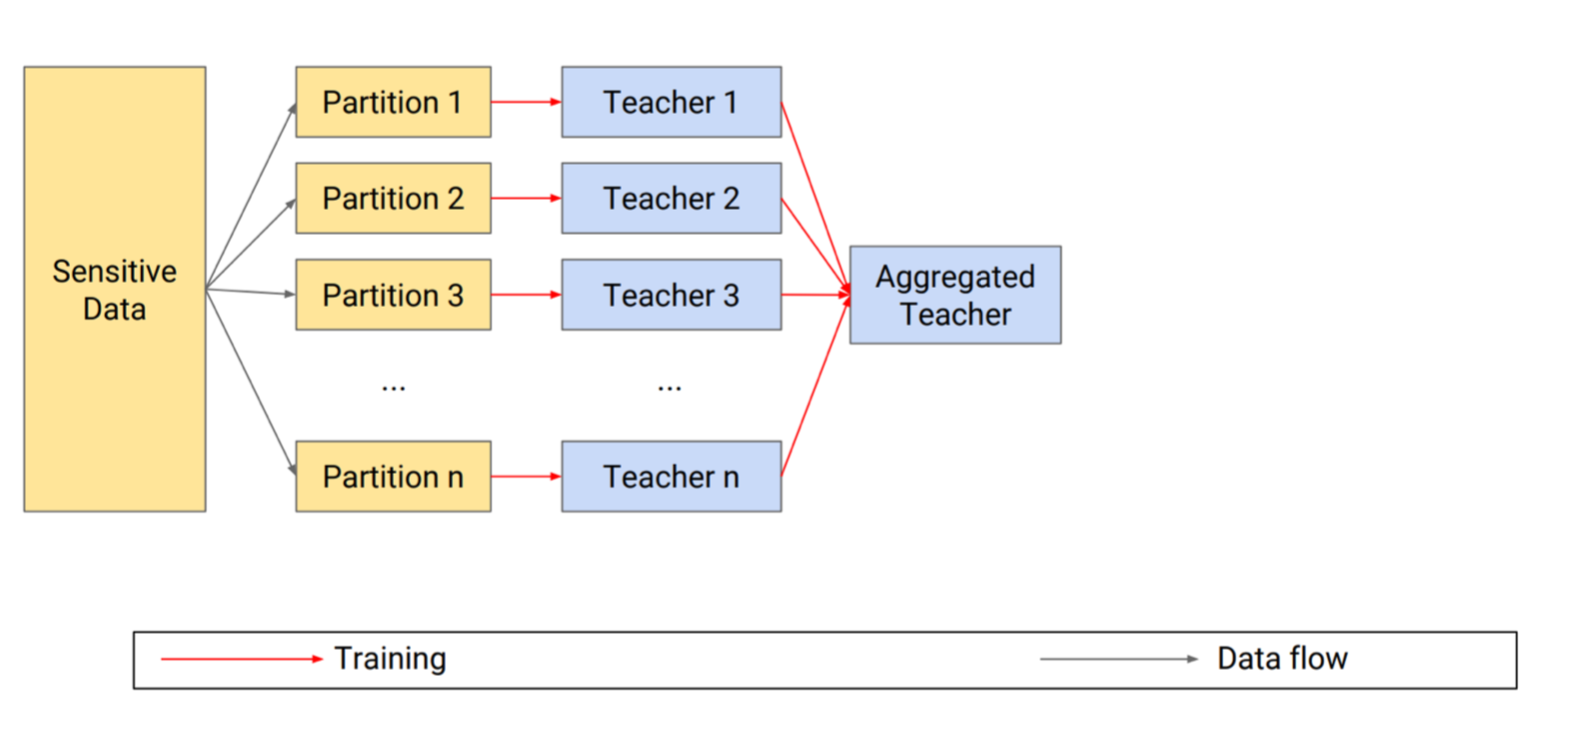
\includegraphics[width = \linewidth]{fig/teacher-model.png}
\caption{教师模型的聚集过程}
\label{fig:teacher-model}
\end{figure}

\begin{figure}[!ht]
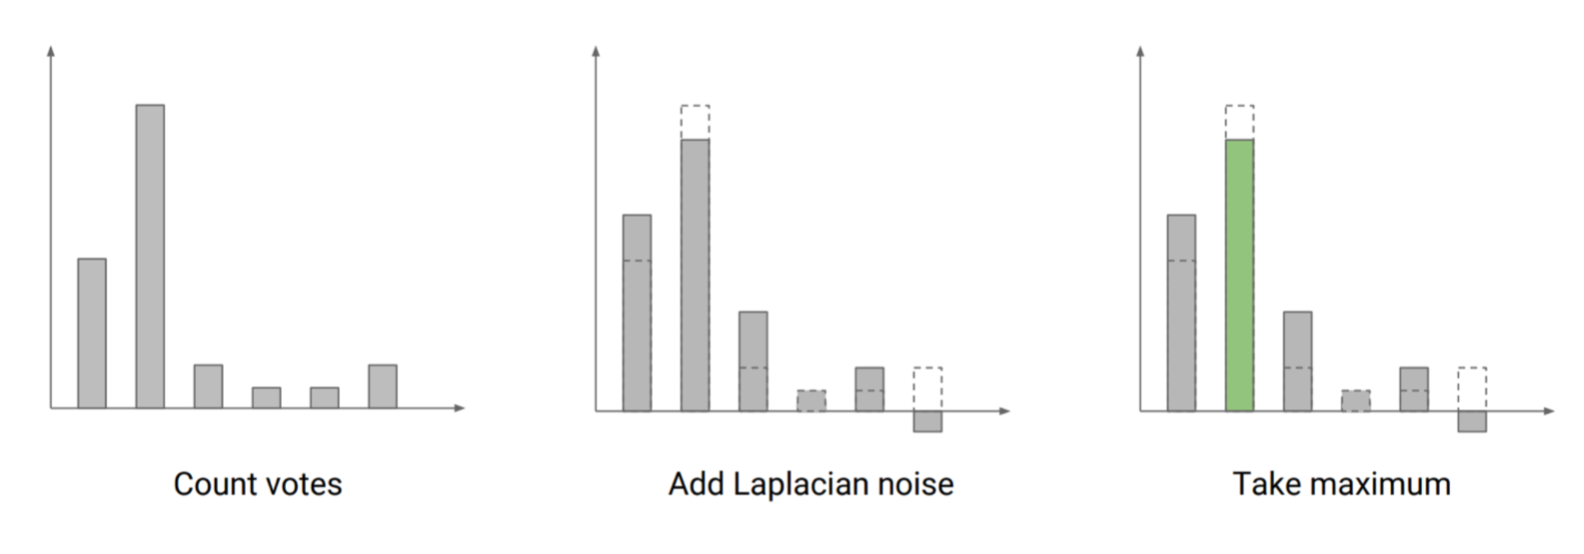
\includegraphics[width = \linewidth]{fig/aggergation.png}
\label{fig:aggergation}
\end{figure}
\begin{itemize}
\item 如果大部分教师模型都同意某一个预测结果,即不依赖于具体的分散数据集,隐私成本很小。
\item 如果有两类预测结果有相近的票数,那么这种不一致,或许会泄露隐私信息。
\end{itemize}


\subsection{学生模型}

\begin{itemize}
\item 聚合教师模型可以看作是一个差分隐私API,用户提交输入值,模型就会返回相应的标签,同时又能保护隐私。
\item 但是,如果训练一个模型,部署到用户设备上直接运行模型得出预测结果,这样的话肯定会更好。为了训练学生模型,需要聚合教师模型以隐私保护的方式,来给公共数据进行标注,传递知识。
\end{itemize}

\begin{figure}[!ht]
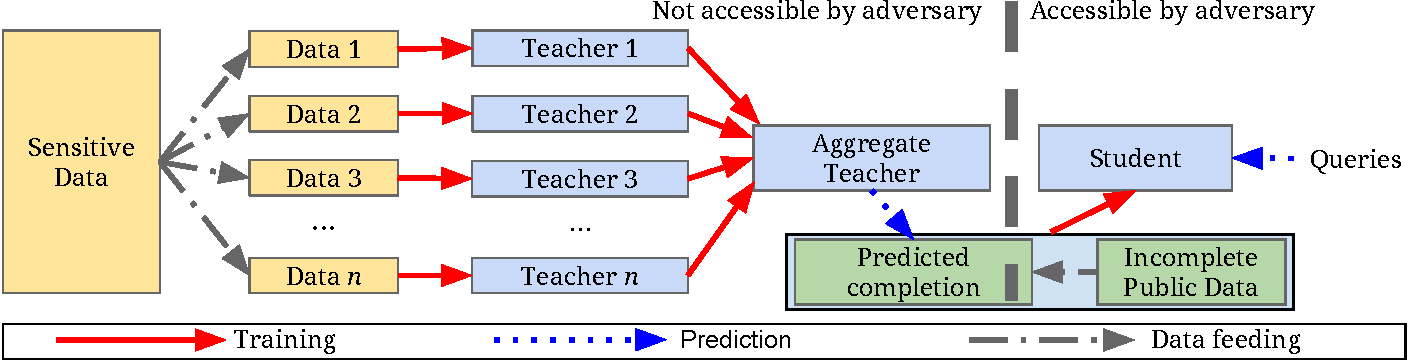
\includegraphics[width = \linewidth]{fig/approach-overview.pdf}
\caption{学生模型的训练}
\label{fig:overview}
\end{figure}
使用未标记的公开数据训练学生模型,部分数据使用对教师模型的查询结果进行标记。



学生模型的必要性:
\begin{enumerate}
\item 每次查询聚合教师模型,都会增加隐私成本。训练学生模型后,只能对聚合教师模型进行固定数量的查询,隐私成本就会被固定下来。
\item 需要防范攻击者探取模型底层函数库。教师模型是由隐私数据训练的,学生模型是由公共数据(非隐私数据)训练的,带有隐私保护的标注。即使攻击者获取到学生模型的训练数据,也只能得到带有隐私保护的标签信息。
\end{enumerate}
总体上:
\begin{itemize}
\item 教师模型用来防御白盒攻击
\item 学生模型用来防御黑盒攻击
\end{itemize}


\section{生成式PATE}

\begin{figure}[!ht]
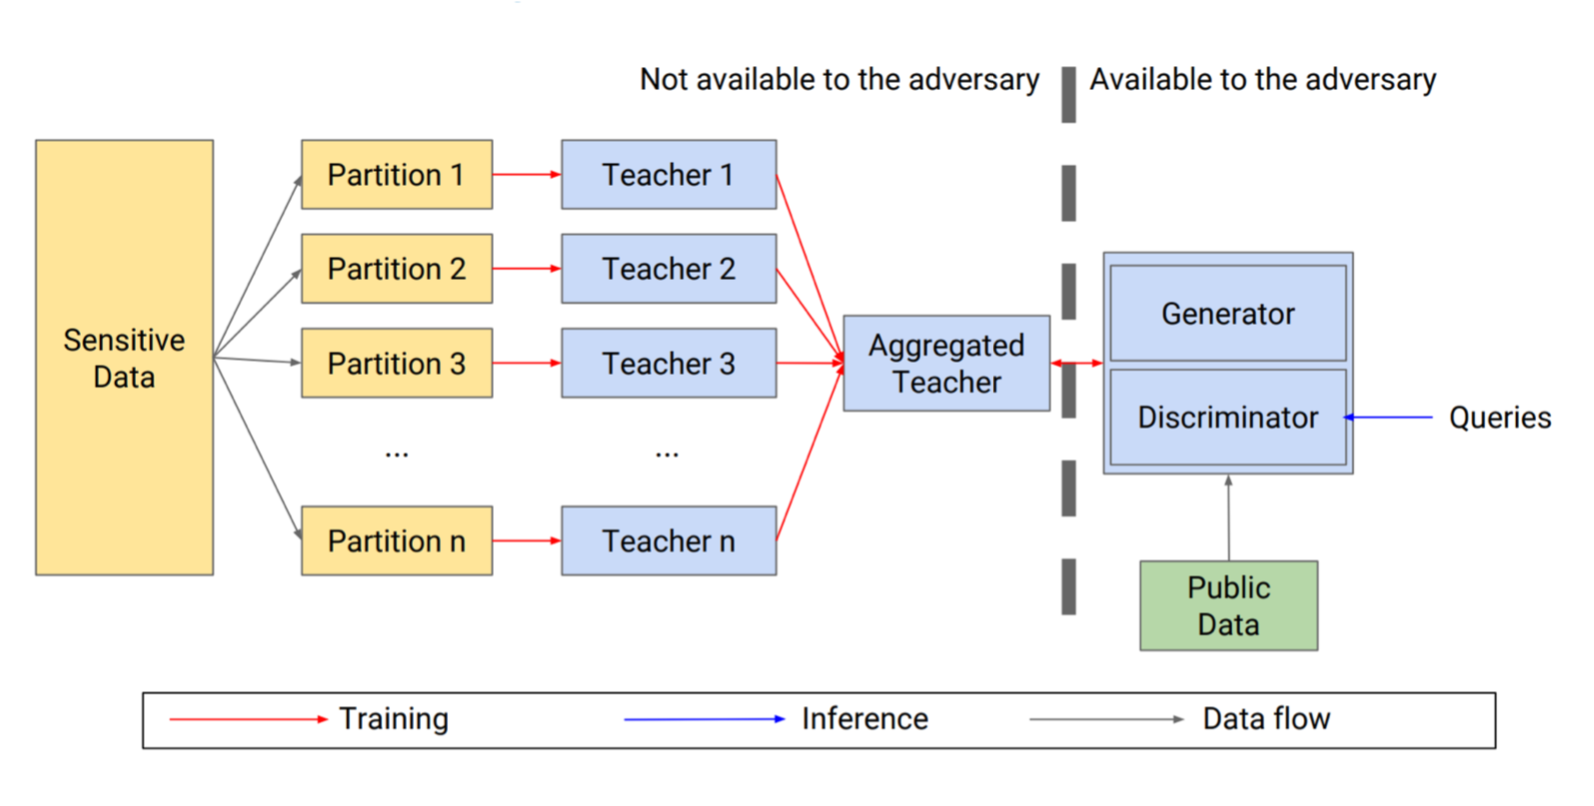
\includegraphics[width = 4in]{fig/student-model-gan.png}
\caption{使用GAN训练学生模型}
\end{figure}
\begin{itemize}
\item 将原本二元分类的判别器扩展至一个多类别的分类器,区分:已标注的真实样本,未标注真实样本,以及生成样本。
\item 训练之后只使用判别器来处理查询。
\end{itemize}


\section{实验}

使用了四个数据集:MNIST、SVHN、UCI Adult 和 UCI Diabetes。如图所示:
\begin{figure}[!ht]
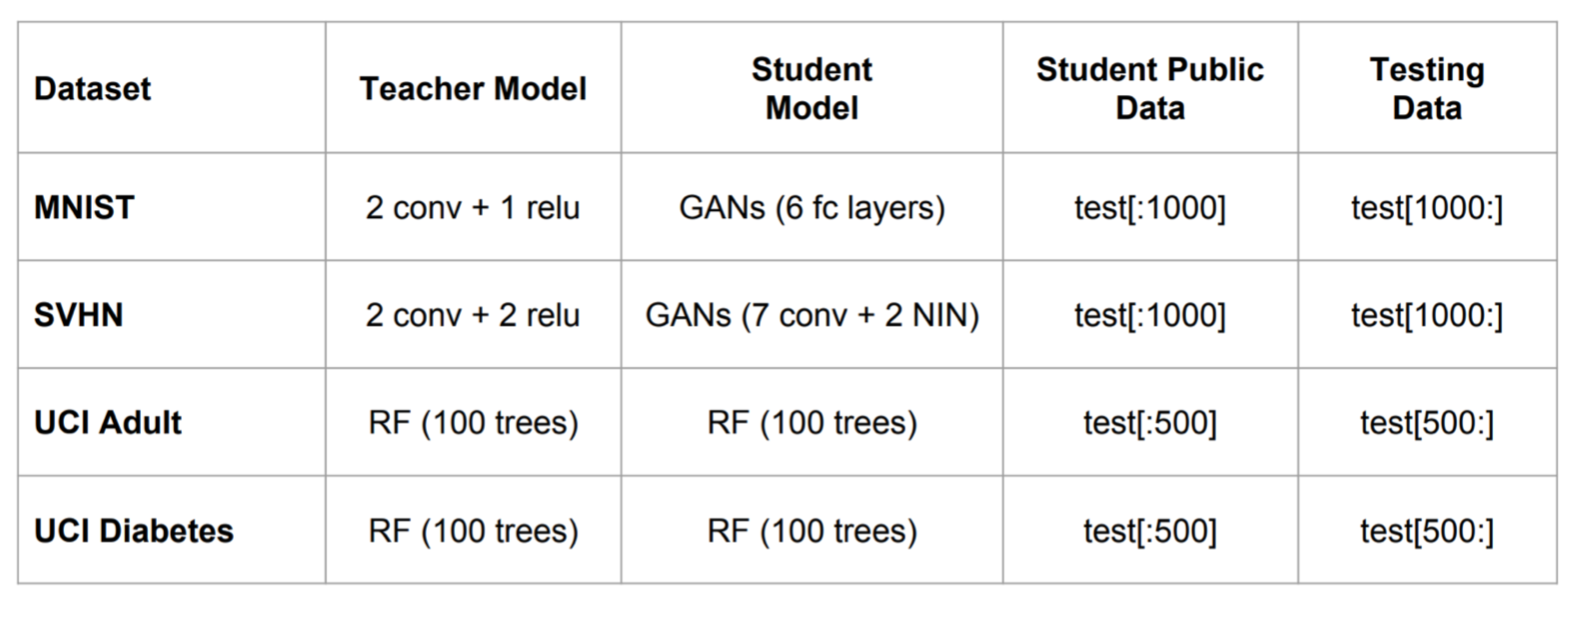
\includegraphics[width = \linewidth]{fig/experiment-settings.png}
\caption{实验数据集}
\end{figure}


\subsection{教师模型准确率}

图\ref{fig:teacher-accuracy}描绘了聚合教师模型的准确率。在训练学生模型之前,需要考虑了每一个标签的隐私。横轴是每一个标签查询的$\epsilon$值,纵轴是预测结果的平均准确率。
\begin{figure}[!ht]
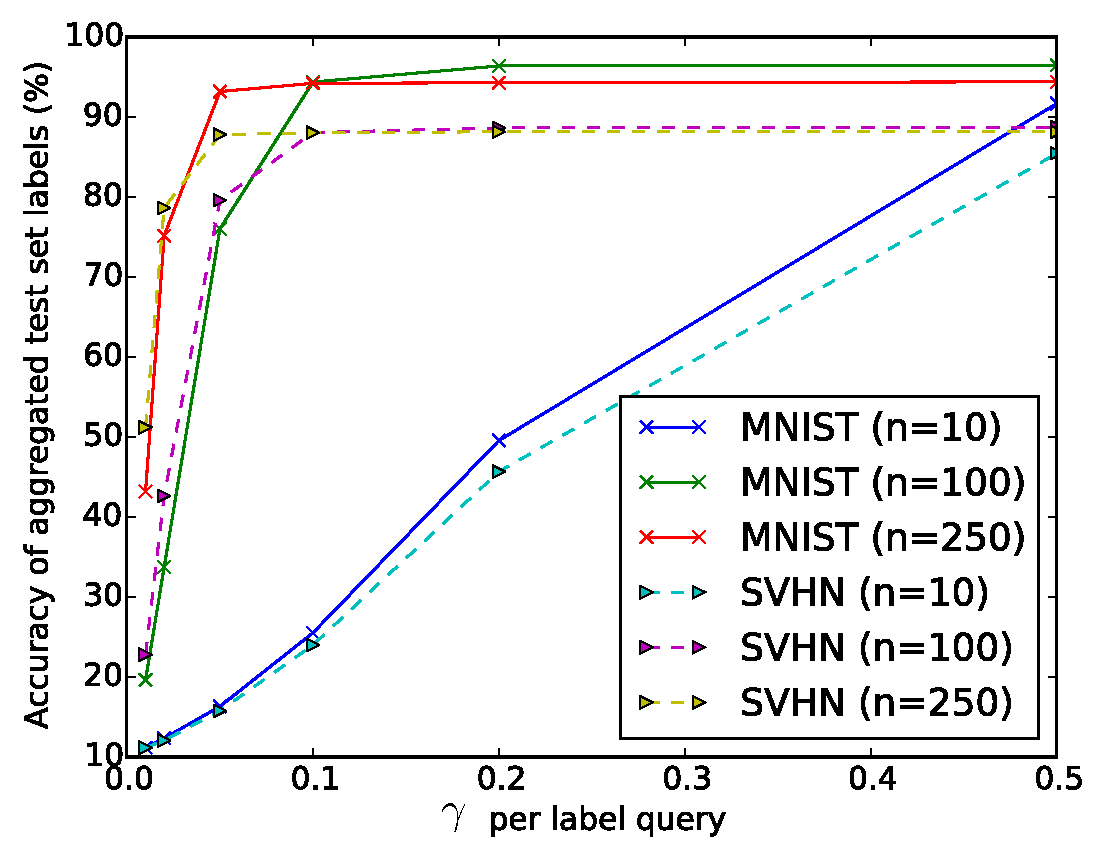
\includegraphics[width = 2.3in]{fig/lap-scale-accuracy.pdf}
\caption{聚合教师模型准确率}
\label{fig:teacher-accuracy}
\caption{紫色的线代表10个聚合教师模型($n=10$)。逐渐降低$\epsilon$值,准确率也很快下降。但如图中绿线和红线的部分,分别包含100个和250个聚合教师模型($n=100, n=250$),在较低$\epsilon$值时,仍可以保持较高的准确率。}
\end{figure}



\subsection{对比}

\begin{figure}[!ht]
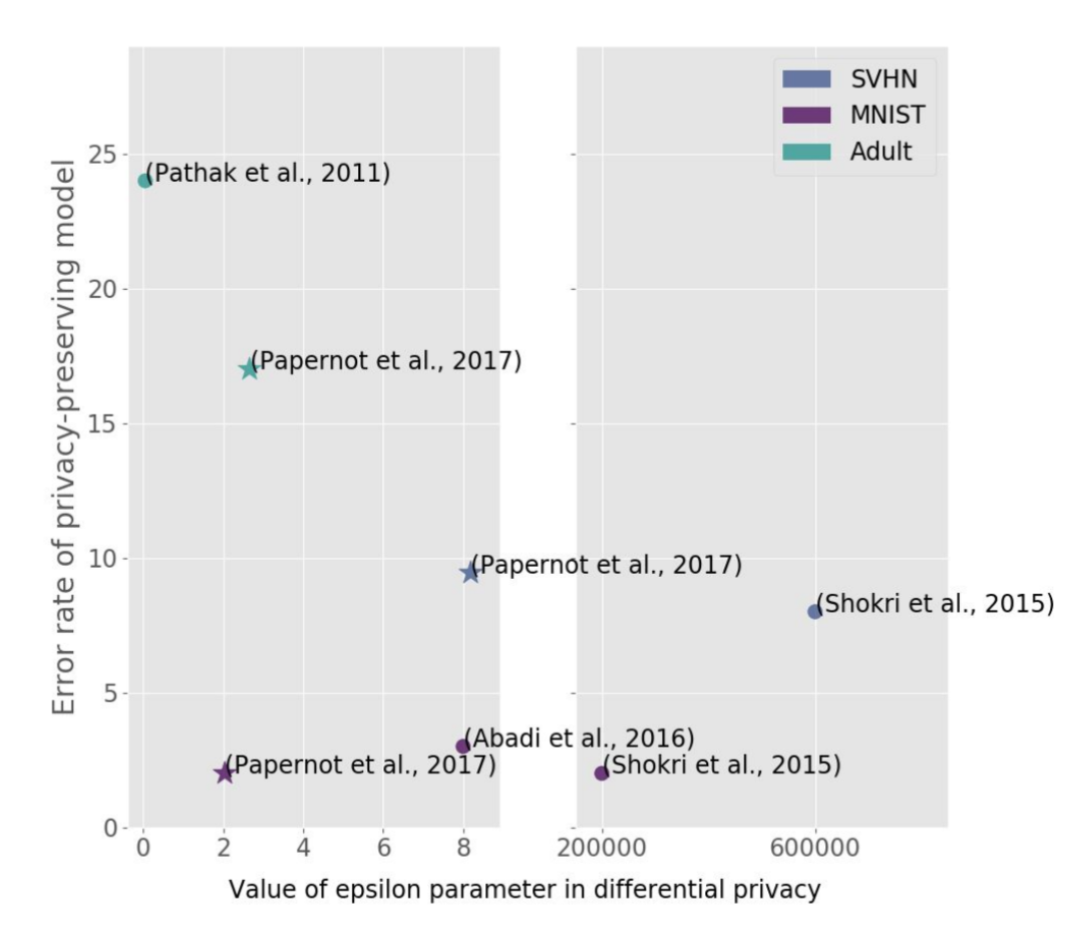
\includegraphics[width = 2.1in]{fig/approach-comparison.png}
\caption{不同Approach的对比}
\end{figure}

\newpage

\bibliography{references}
\bibliographystyle{IEEEtran}


\end{document}
